\documentclass[11pt,a4paper]{article}
\newcommand{\intestazione}{Trimero ad anello --- 8. I correlatori sotto rumore}
% =====================================================================
%  Preambolo comune ai documenti sul dimero (serie "che cosa abbiamo fatto")
%  Incluso con % =====================================================================
%  Preambolo comune ai documenti sul dimero (serie "che cosa abbiamo fatto")
%  Incluso con % =====================================================================
%  Preambolo comune ai documenti sul dimero (serie "che cosa abbiamo fatto")
%  Incluso con \input{preambolo_dimero} subito dopo \documentclass.
% =====================================================================
\usepackage[T1]{fontenc}
\usepackage[utf8]{inputenc}
\usepackage[main=italian,provide=*]{babel}
\usepackage{amsmath,amssymb,mathtools}
\usepackage{graphicx}
\usepackage{booktabs}
\usepackage{colortbl}
\usepackage{xcolor}
\usepackage{geometry}
\usepackage{placeins}
\usepackage{caption}
\usepackage{enumitem}
\usepackage{fancyhdr}
\usepackage{needspace}
\usepackage{tikz}
\usetikzlibrary{arrows.meta,positioning,shapes.geometric,calc,fit,backgrounds}
\usepackage{hyperref}
\hypersetup{colorlinks=true,linkcolor=blu,citecolor=blu,urlcolor=blu}

\geometry{margin=2.5cm}

% --- colori coerenti con quelli delle figure (palette Okabe-Ito)
\definecolor{blu}{HTML}{0072B2}
\definecolor{arancio}{HTML}{E69F00}
\definecolor{verdes}{HTML}{009E73}
\definecolor{rossos}{HTML}{D55E00}
\definecolor{violas}{HTML}{CC79A7}
\definecolor{grigetto}{HTML}{E8E8E8}

\captionsetup{font=small,labelfont=bf,width=0.92\textwidth}

\pagestyle{fancy}
\fancyhf{}
\fancyhead[L]{\small\itshape\intestazione}
\fancyhead[R]{\small\thepage}
\renewcommand{\headrulewidth}{0.3pt}

% --- notazione
\newcommand{\ket}[1]{\lvert #1\rangle}
\newcommand{\bra}[1]{\langle #1 \rvert}
\newcommand{\media}[1]{\langle #1 \rangle}
\newcommand{\vs}[1]{\mathbf{s}_{#1}}

% --- riquadro "in una riga": il messaggio da portare a casa
\newcommand{\messaggio}[1]{%
  \begin{center}
  \begin{minipage}{0.93\textwidth}
  \setlength{\fboxsep}{9pt}%
  \colorbox{grigetto}{\begin{minipage}{\dimexpr\textwidth-2\fboxsep}
  \small\textbf{In una riga.}\enspace #1
  \end{minipage}}
  \end{minipage}
  \end{center}
}

% --- riquadro "come lo sappiamo": la verifica numerica dietro un'affermazione
\newcommand{\verifica}[1]{%
  \begin{center}
  \begin{minipage}{0.93\textwidth}
  \small\textcolor{verdes}{\rule{2.2em}{1.1pt}}\enspace
  \textcolor{verdes}{\textbf{Come lo sappiamo.}}\enspace #1
  \end{minipage}
  \end{center}
  \medskip
}
 subito dopo \documentclass.
% =====================================================================
\usepackage[T1]{fontenc}
\usepackage[utf8]{inputenc}
\usepackage[main=italian,provide=*]{babel}
\usepackage{amsmath,amssymb,mathtools}
\usepackage{graphicx}
\usepackage{booktabs}
\usepackage{colortbl}
\usepackage{xcolor}
\usepackage{geometry}
\usepackage{placeins}
\usepackage{caption}
\usepackage{enumitem}
\usepackage{fancyhdr}
\usepackage{needspace}
\usepackage{tikz}
\usetikzlibrary{arrows.meta,positioning,shapes.geometric,calc,fit,backgrounds}
\usepackage{hyperref}
\hypersetup{colorlinks=true,linkcolor=blu,citecolor=blu,urlcolor=blu}

\geometry{margin=2.5cm}

% --- colori coerenti con quelli delle figure (palette Okabe-Ito)
\definecolor{blu}{HTML}{0072B2}
\definecolor{arancio}{HTML}{E69F00}
\definecolor{verdes}{HTML}{009E73}
\definecolor{rossos}{HTML}{D55E00}
\definecolor{violas}{HTML}{CC79A7}
\definecolor{grigetto}{HTML}{E8E8E8}

\captionsetup{font=small,labelfont=bf,width=0.92\textwidth}

\pagestyle{fancy}
\fancyhf{}
\fancyhead[L]{\small\itshape\intestazione}
\fancyhead[R]{\small\thepage}
\renewcommand{\headrulewidth}{0.3pt}

% --- notazione
\newcommand{\ket}[1]{\lvert #1\rangle}
\newcommand{\bra}[1]{\langle #1 \rvert}
\newcommand{\media}[1]{\langle #1 \rangle}
\newcommand{\vs}[1]{\mathbf{s}_{#1}}

% --- riquadro "in una riga": il messaggio da portare a casa
\newcommand{\messaggio}[1]{%
  \begin{center}
  \begin{minipage}{0.93\textwidth}
  \setlength{\fboxsep}{9pt}%
  \colorbox{grigetto}{\begin{minipage}{\dimexpr\textwidth-2\fboxsep}
  \small\textbf{In una riga.}\enspace #1
  \end{minipage}}
  \end{minipage}
  \end{center}
}

% --- riquadro "come lo sappiamo": la verifica numerica dietro un'affermazione
\newcommand{\verifica}[1]{%
  \begin{center}
  \begin{minipage}{0.93\textwidth}
  \small\textcolor{verdes}{\rule{2.2em}{1.1pt}}\enspace
  \textcolor{verdes}{\textbf{Come lo sappiamo.}}\enspace #1
  \end{minipage}
  \end{center}
  \medskip
}
 subito dopo \documentclass.
% =====================================================================
\usepackage[T1]{fontenc}
\usepackage[utf8]{inputenc}
\usepackage[main=italian,provide=*]{babel}
\usepackage{amsmath,amssymb,mathtools}
\usepackage{graphicx}
\usepackage{booktabs}
\usepackage{colortbl}
\usepackage{xcolor}
\usepackage{geometry}
\usepackage{placeins}
\usepackage{caption}
\usepackage{enumitem}
\usepackage{fancyhdr}
\usepackage{needspace}
\usepackage{tikz}
\usetikzlibrary{arrows.meta,positioning,shapes.geometric,calc,fit,backgrounds}
\usepackage{hyperref}
\hypersetup{colorlinks=true,linkcolor=blu,citecolor=blu,urlcolor=blu}

\geometry{margin=2.5cm}

% --- colori coerenti con quelli delle figure (palette Okabe-Ito)
\definecolor{blu}{HTML}{0072B2}
\definecolor{arancio}{HTML}{E69F00}
\definecolor{verdes}{HTML}{009E73}
\definecolor{rossos}{HTML}{D55E00}
\definecolor{violas}{HTML}{CC79A7}
\definecolor{grigetto}{HTML}{E8E8E8}

\captionsetup{font=small,labelfont=bf,width=0.92\textwidth}

\pagestyle{fancy}
\fancyhf{}
\fancyhead[L]{\small\itshape\intestazione}
\fancyhead[R]{\small\thepage}
\renewcommand{\headrulewidth}{0.3pt}

% --- notazione
\newcommand{\ket}[1]{\lvert #1\rangle}
\newcommand{\bra}[1]{\langle #1 \rvert}
\newcommand{\media}[1]{\langle #1 \rangle}
\newcommand{\vs}[1]{\mathbf{s}_{#1}}

% --- riquadro "in una riga": il messaggio da portare a casa
\newcommand{\messaggio}[1]{%
  \begin{center}
  \begin{minipage}{0.93\textwidth}
  \setlength{\fboxsep}{9pt}%
  \colorbox{grigetto}{\begin{minipage}{\dimexpr\textwidth-2\fboxsep}
  \small\textbf{In una riga.}\enspace #1
  \end{minipage}}
  \end{minipage}
  \end{center}
}

% --- riquadro "come lo sappiamo": la verifica numerica dietro un'affermazione
\newcommand{\verifica}[1]{%
  \begin{center}
  \begin{minipage}{0.93\textwidth}
  \small\textcolor{verdes}{\rule{2.2em}{1.1pt}}\enspace
  \textcolor{verdes}{\textbf{Come lo sappiamo.}}\enspace #1
  \end{minipage}
  \end{center}
  \medskip
}


\title{\bfseries Quando il rumore incontra una misura vera\\[2pt]
\large Documento 8 --- correlatori rumorosi, readout a shot finiti}
\author{Samuele Schiavi \\ \small Tesi triennale in Fisica, Università di Parma
--- Relatore: Prof.\ Alessandro Chiesa}
\date{}

\begin{document}
\maketitle
\thispagestyle{fancy}

\section{Una differenza qualitativa rispetto ai due documenti precedenti}

Il VQE (Documento 6) e la dinamica (Documento 7) non richiedono mai una
misura: energia e fedeltà si leggono direttamente sull'operatore densità.
Il correlatore dinamico no --- serve misurare l'ancilla, e una misura reale
porta con sé il readout, non solo il rumore di gate.

\section{Il circuito, con il rumore su ogni ingrediente}

Stesso schema Hadamard test della Parte 1 (Documento 4), quattro qubit,
ma ora ogni gate --- preparazione, controllo, Trotter, anti-controllo ---
attraversa il canale depolarizzante, e la misura finale sull'ancilla porta
un errore di lettura vero.

\begin{figure}[htbp]
\centering
\begin{minipage}{0.48\textwidth}
\centering
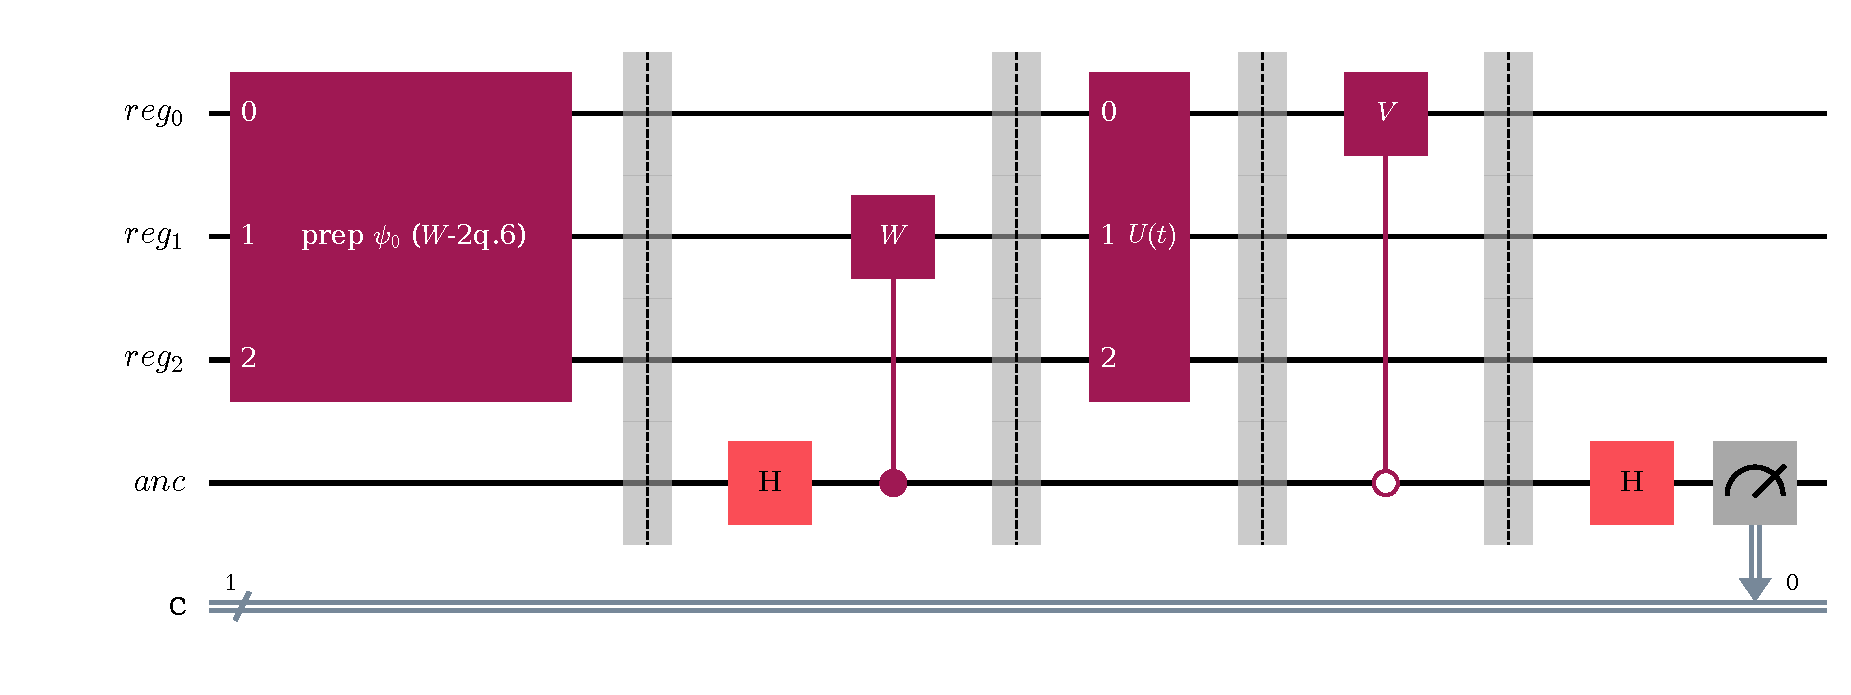
\includegraphics[width=\textwidth]{figure/circ_correlatore_schema_re_anello}
\\ parte reale
\end{minipage}
\hfill
\begin{minipage}{0.48\textwidth}
\centering
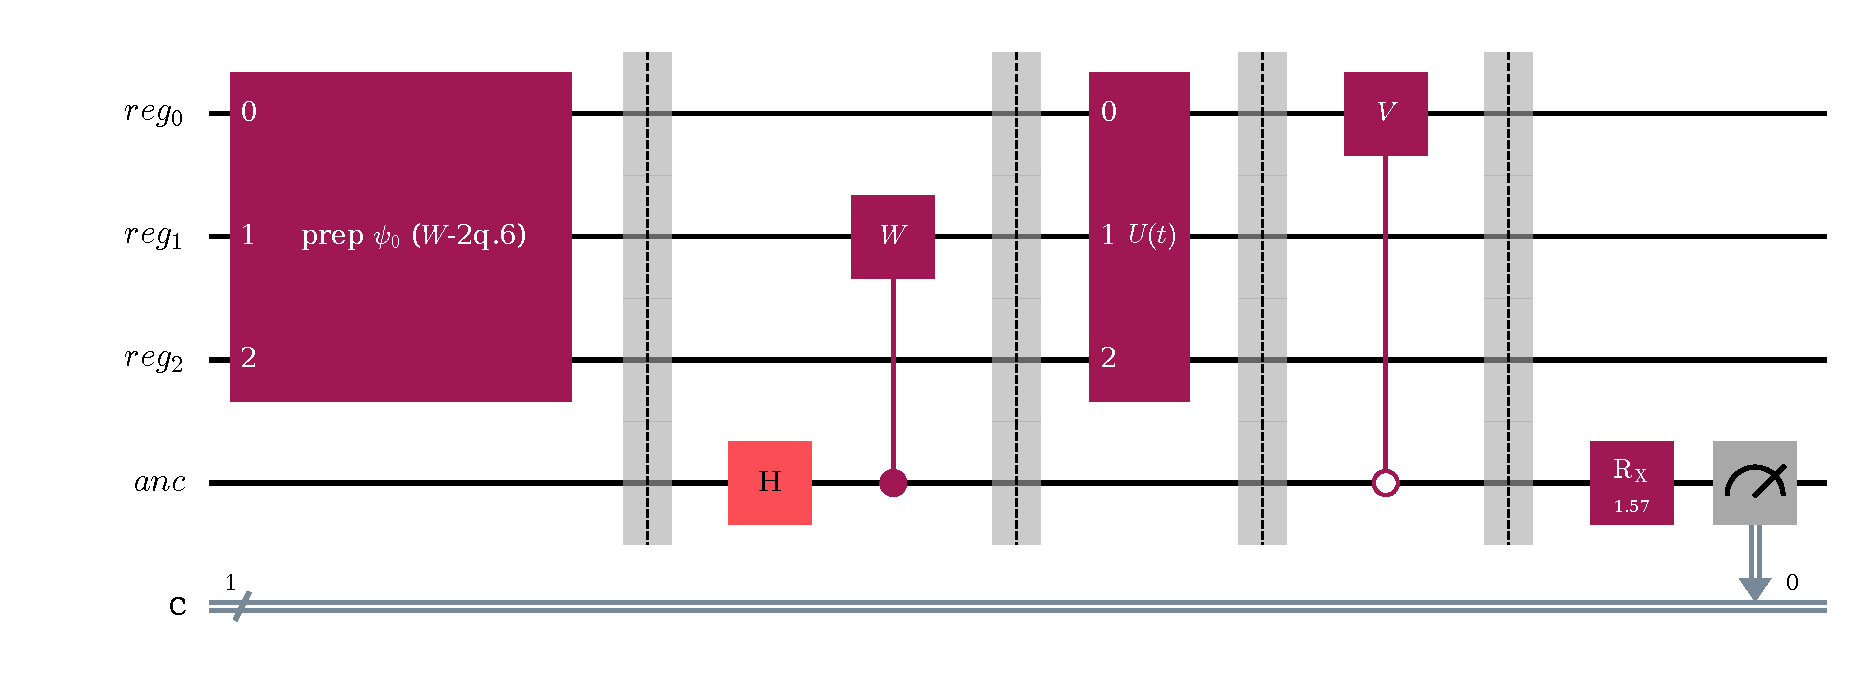
\includegraphics[width=\textwidth]{figure/circ_correlatore_schema_im_anello}
\\ parte immaginaria
\end{minipage}
\caption{Schema del circuito (non transpilato, per leggibilità). Le due
varianti differiscono solo nella rotazione finale sull'ancilla prima della
misura --- $H$ per la parte reale, $R_x(\pi/2)$ per l'immaginaria.}
\end{figure}
\FloatBarrier

\section{Quale correlatore, e perché}

$C_{21}^{xx}(t{=}2)$, punto di lavoro Scenario A ($b/J=2.4$, $D/J=0.15$,
Opzione DM B) --- lo stesso già usato come baseline nello Stadio 4
della pipeline originaria di questa Parte 2, verificato non fragile (posizione
64°/81 per robustezza del segnale su tutte le combinazioni, controllato in
una sessione precedente di questo stesso progetto): non l'estremo più
debole, una scelta rappresentativa.

\section{Il readout: misura genuina, non una formula}

A differenza della pipeline originaria di questa Parte 2 sull'anello (dove
il readout era una correzione analitica, $(1-2p)\langle Z\rangle_\text{ideale}$,
applicata dopo la simulazione del rumore di gate), qui il readout è
\textbf{genuinamente campionato}: un \texttt{ReadoutError} vero agganciato
al simulatore, misura a shot finiti ($10^5$ shot per punto), nessuna
formula.

\verifica{Confronto diretto formula analitica contro shot finiti, stesso
punto di riferimento: $N=3$, analitico $-0.4710+0.1816i$, shot finiti
$-0.4715+0.1826i$ --- scarto $1.15\times10^{-3}$, coerente con l'errore
statistico atteso per $2\times10^5$ shot ($\sim1/\sqrt{2\times10^5}\approx
2.2\times10^{-3}$).}

\section{Risultato: la curva $|C(N)|$ e $N^*$}

\begin{figure}[htbp]
\centering
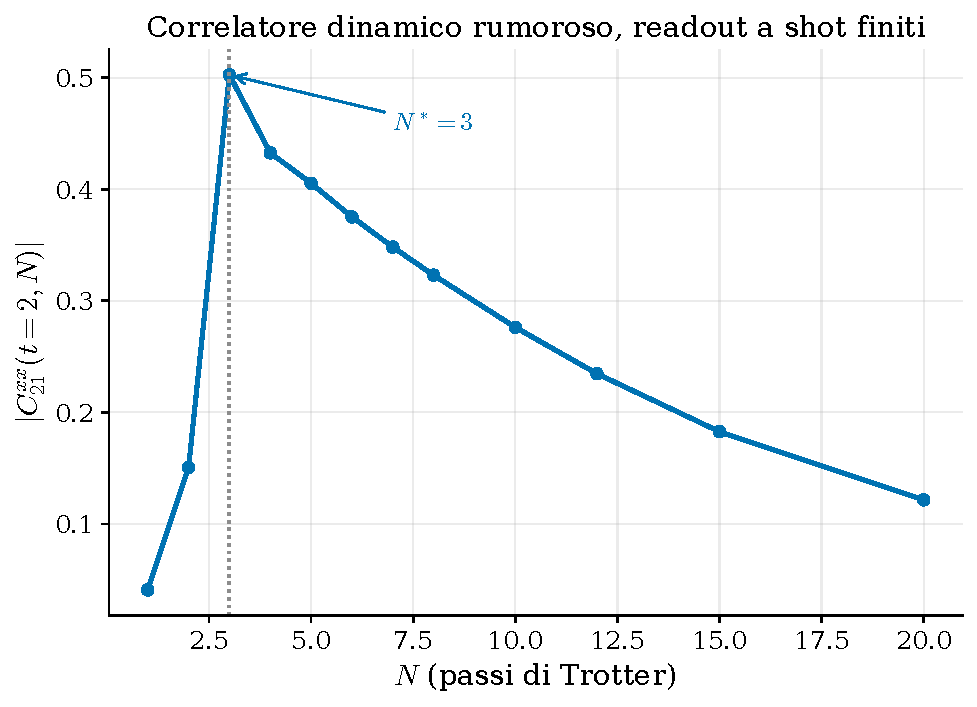
\includegraphics[width=0.68\textwidth]{figure/fig_passo4_correlatore_vs_N_anello}
\caption{$|C_{21}^{xx}(t{=}2,N)|$, rumore di riferimento, readout a shot
finiti ($10^5$ shot per punto). $N^*=3$, $|C(N^*)|=0.5026$.}
\end{figure}
\FloatBarrier

$N^*=3$ coincide esattamente con il valore già stabilito con la formula
analitica ($N^*=3$, $|C(N^*)|=0.5048$) --- lo scarto sul valore di picco è
coerente con l'errore statistico atteso.

\section{Un confronto col dimero: qui $N^*$ \emph{non} sovrastima il vero valore}

Sul dimero, un chiarimento importante (Documento 8 gemello): $|C(N^*)|$
sovrastimava il correlatore fisico vero di quasi il doppio --- $N^*$
massimizza il segnale misurabile, non l'accuratezza della stima. Vale la
pena controllare se lo stesso vale qui, non assumerlo per analogia.

\begin{table}[htbp]
\centering
\small
\renewcommand{\arraystretch}{1.3}
\begin{tabular}{@{}lccc@{}}
\toprule
\rowcolor{grigetto}
\textbf{Livello} & $N^*$ & $|C|$ & \textbf{rapporto a $C_\text{esatto}$} \\
\midrule
$C_\text{esatto}(t{=}2)$\footnotemark[1] --- nessun Trotter, nessun rumore & --- & $0.6723$ & $1.00\times$ \\
$C(N;t{=}2)$, rumore nullo (solo Trotter) & $3$ & $0.6773$ & $1.007\times$ \\
$C(N;t{=}2)$, rumore vero (Trotter + gate + lettura) & $3$ & $0.5026$ & $0.748\times$ \\
\bottomrule
\end{tabular}
\caption{I tre livelli per il correlatore $C_{21}^{xx}$, Scenario A.}
\end{table}
\footnotetext[1]{``Esatto'' qui vuol dire \emph{calcolato numericamente
senza approssimazioni fisiche}, non una formula chiusa: diagonalizzazione
diretta della matrice $8\times8$ (\texttt{np.linalg.eigh}) per
$\ket{\psi_0}$, esponenziale di matrice diretto
(\texttt{scipy.linalg.expm}) per $U(t)=e^{-iHt}$ --- nessun Trotter,
nessun canale di rumore. L'unica imprecisione è l'arrotondamento in
virgola mobile ($\sim10^{-14}$), trascurabile rispetto alle differenze
del $25$--$75\%$ qui discusse.}

\verifica{$C_\text{esatto}(t{=}2)$, somma spettrale diretta (nessun
Trotter, nessun rumore): $\lvert C_\text{esatto}\rvert=0.6723$. A rumore
nullo, $N^*=3$ dà $\lvert C(N^*)\rvert=0.6773$ --- \textbf{praticamente
coincidente} col vero valore, non quasi il doppio. Sotto rumore di
riferimento, $\lvert C(N^*)\rvert=0.5026$ --- più \emph{basso} del vero
valore, non più alto.}

\messaggio{Il fenomeno scoperto sul dimero (sovrastima sistematica da parte
di $N^*$) \textbf{non si ripete qui}, almeno per questo correlatore e questo
punto di lavoro. Non è una contraddizione: è la conferma che quel fenomeno
dipendeva dalla combinazione specifica di errore di Trotter e forma della
curva sul dimero, non è una proprietà universale di $N^*=\arg\max_N|C(N)|$.
Ogni nuovo sistema va controllato di persona, anche quando un fenomeno
analogo era già stato trovato altrove.}

\paragraph{La differenza col dimero, ora visibile riga per riga.} Sul
dimero, a rumore nullo $N^*$ sovrastima $C_\text{esatto}$ di quasi il
doppio ($0.5894$ contro $0.3177$, $\sim1.86\times$). Sull'anello, a
rumore nullo, $N^*$ è già praticamente coincidente col vero valore fisico
($1.007\times$, non $1.86\times$) --- il rumore poi lo riporta
\emph{sotto} il valore esatto ($0.748\times$), non sopra. Stesso schema a
tre righe (esatto, rumore nullo, rumore vero), esito qualitativamente
diverso sulla riga di mezzo.

\section{Il conteggio dei gate cresce come deve}

Il circuito dei correlatori resta il più lungo di tutta la pipeline
dell'anello: preparazione ($6$ CNOT) più $N=3$ passi di Trotter ($15$ CNOT
ciascuno, $45$ in tutto) più le due porte controllate sull'ancilla ---
oltre $50$ CNOT nel circuito completo al punto di lavoro di riferimento.

\end{document}
